%!TEX root = ../template.tex
%%%%%%%%%%%%%%%%%%%%%%%%%%%%%%%%%%%%%%%%%%%%%%%%%%%%%%%%%%%%%%%%%%%%
%% chapter4.tex
%% NOVA thesis document file
%%
%% Chapter with lots of dummy text
%%%%%%%%%%%%%%%%%%%%%%%%%%%%%%%%%%%%%%%%%%%%%%%%%%%%%%%%%%%%%%%%%%%%

\typeout{NT FILE chapter4.tex}%

\chapter{Implementação e Plano de Trabalho}
\label{cha:abordagem_plano}

Neste capítulo vai ser apresentada a proposta de abordagem para a segunda fase da dissertação bem como o diagrama Gantt que a suporta. 

\section{Processo de Desenvolvimento} % (fold) antigo Tecnologias e Processo de Desenvolvimento
\label{sec:tecnologias_processo}

Para a segunda fase da dissertação, será tomada uma abordagem iterativa para a implementação da ferramenta Dashboard Designer. Esta etapa terá como principal objetivo o desenvolvimento de uma aplicação \textit{web} funcional e interativa que permita aos seus utilizadores modelar diferentes \textit{dashboards} de forma eficiente e intuitiva.

O desenvolvimento da ferramenta será feito através da realização de \textit{sprints} semanais. Cada \textit{sprint} terá metas e objetivos específicos, correspondentes à implementação de diferentes subconjuntos de funcionalidades que a ferramenta irá possuir. Através deste planeamento estratégico, é feito um controlo rigoroso sobre a evolução da aplicação, facilitando a deteção de problemas, atrasos e imprevistos durante a sua implementação.

Ao terminar o desenvolvimento funcional da ferramenta, é dado ínicio ao processo de avaliação da mesma com utilizadores reais, com o objetivo de avaliar a usabilidade da solução desenvolvida. Para a avaliação, vão ser selecionados utilizadores com perfis adequados, isto é, utilizadores com experiência ou interesse na área de visualização de dados, que serão convidados a implementar diferentes tarefas. Estes utilizadores serão selecionados através de redes de contactos próximos ou através de comunidades \textit{online} fidedignas. Estas tarefas permitem identificar a forma como os utilizadores interagem com a ferramenta, facilitando a identificação de eventuais dificuldades ou imprevistos na sua realização.

Após a realização dos testes de usabilidade com os diferentes utilizadores, os resultados obtidos são recolhidos e analisados de forma sistemática. Esta análise permite identificar os pontos fortes e fracos da ferramenta, identificando as dificuldades mais recorrentes, erros de interação e funcionalidades pouco intuitivas. Com base nos padrões de análise recolhidos, serão definidas medidas de melhoria da ferramenta sempre que necessário. Desta forma, é possível garantir que a versão final da solução desenvolvida é fundamentada e centrada na experiência do utilizador.

\section{Plano de Trabalho} % (fold)
\label{sec:plano_trabalho}

De forma a alcançar os objetivos estipulados para a realização do trabalho, foi elaborado um diagrama de Gantt apresentado na Tabela~\ref{tab:ganttchart}. Este diagrama apresenta a estimativa do tempo a desenvolver as atividades pretendidas, no entanto, é importante realçar que o mesmo pode vir a sofrer alterações no decorrer da sua implementação.

\begin{figure}[htbp]
  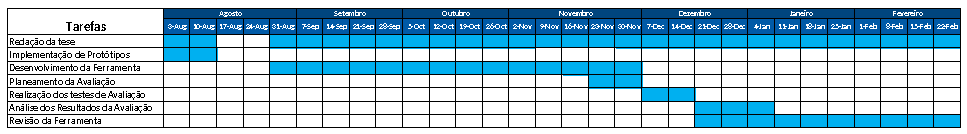
\includegraphics[width=\textwidth]{diagramas/Gantt_Semanal (4)_cropped}
  \centering
  \caption{Diagrama de Gantt.}
  \label{tab:ganttchart}
\end{figure}

A tarefa de \textbf{Implementação de Protótipos} está prevista para ser realizada durante as primeiras duas semanas de agosto. Esta tarefa corresponde à criação de versões iniciais e reais do \textit{layout} da ferramenta. A realização de diferentes protótipos oferece a possibilidade de experimentar diferentes abordagens a nível visual e funcional.

Após a relização dos protótipos, é iniciado o \textbf{Desenvolvimento da Ferramenta} com duração até ínicio de dezembro, onde irá ser desenvolvida de forma iterativa a versão funcional da aplicação do Dashboard Designer. 

No final de novembro, irá ser realizada a tarefa de \textbf{Planeamento de Avaliação}, essencial para estruturar a fase de avaliação da solução desenvolvida. Nesta fase, vai ser feito o planeamento das atividades e métricas a serem avaliadas, bem como os testes que irão ser implementados de forma a testar todas as funcionalidades propostas pela ferramenta.

A tarefa de \textbf{Realização dos Testes de Avaliação} será realizada no ínicio do mês de dezembro, e representa a fase de testes com utilizadores reais. Durante esta fase, os utilizadores serão convidados a realizar as tarefas estipuladas no planeamento da avaliação, com o objetivo de avaliar a usabilidade e a eficácia da ferramenta desenvolvida.

A tarefa de \textbf{Análise de Resultados} será realizada entre meio de dezembro e ínicio de janeiro, e vai consistir na interpretação crítica dos dados recolhidos. Aqui, aspetos como usabilidade, clareza e interpretação vão ser avaliados, com o objetivo de compreender em que medida a ferramenta desenvolvida atinge os objetivos estipulados.

Com base nos resultados obtidos, será realizada a \textbf{Revisão da Ferramenta}, agendada para ter início ao mesmo tempo que a tarefa de análise de resultados. Esta tarefa resulta numa melhoria da solução desenvolvida, tendo em análise os resultados obtidos na fase de análise de resultados.

Para finalizar, a \textbf{Redação da Tese} decorrerá ao longo de toda a segunda fase da dissertação, desta forma, é possível documentar o progresso do trabalho realizado à medida que o mesmo é desenvolvido.